
\documentclass[a4paper,12pt]{book}
\usepackage[latin1]{inputenc}
\usepackage{amsmath}
\usepackage{amsfonts}
\usepackage{amssymb}
\usepackage{makeidx}
\usepackage{apalike}
%\usepackage[brazil]{babel}
\usepackage{graphicx, subfigure} 
\usepackage{listings}  
\usepackage{lettrine} 
\usepackage{url}
%Traduzindo o listings
%\renewcommand{\lstlistingname}{Listagem}
%\renewcommand{\lstlistlistingname}{Listagens}
\author{Cl�udia Torres Code�o \and Fl�vio Code�o Coelho}
\title{EpiGrass User Guide}
\date{Draft}


\makeindex

\begin{document}



\maketitle



{\large
\textbf{EpiGrass is a CNPq funded Project. Participants of this project are:}
\begin{flushright}
Maria Goreti Freitas Rosas (Fiocruz - IOC)\\
Alexios Zavras (Univ of Athenas)\\ 
Pantelis Tsouris (Univ of Athenas)\\
Igor Cabral Correa (Fiocruz - PROCC)\\
Oswaldo Gon�alves Cruz (Fiocruz - PROCC)\\
Flavio Code�o Coelho (Fiocruz - PROCC)\\
Cl�udia Torres Code�o (Fiocruz-PROCC)\\
\end{flushright} 
}



\frontmatter
\lstset{language=csh, numbers=left, numberstyle=\tiny, numbersep=7pt, showstringspaces=false, breaklines}
\chapter{Preface}
\lettrine{T}{he} emergence and re-emergence of infectious diseases and the evolution of resistant pathogens pose a great challenge for Public Health worldwide. Brazil, in particular, is facing increasing problems with the expansion, to urban centers, of diseases previously rural  (leishmaniosis), increasing mortality caused by previously benign diseases (dengue), potencial emergence of new diseases, and reduction of efficacy of traditional treatment protocols (tuberculosis, malaria, leprosy).

To deal with this situation, it is necessary to think strategically. How can we use our limited resources the best way possible? In other words, how to define public health policies for the use of chemicals and vaccines that optimize their impact in the short and long term? To develop such strategies, it is necessary to consider, and integrate, information from different sources, including biological information regarding host-parasite interaction, parasite response to chemicals or other control element, identification of risk situations for the population under study, identification of alternative control strategies, quantification of available resources, etc. The integration of all these data is often done in an incomplete way, resulting in sub-optimal decision making.

Important for the control of infectious diseases is the characterization of the temporal and spatial distribution of cases and risk factors. Climate, topography, human and vector population density are some features that may restrict diseases to certain geographical areas or seasons. In EpiGrass, the georefered space is the background for simulating intervention scenarios. Computer simulations are more and more used for evaluation of risk and formulation of disease control strategies \cite{EACasmanandBFischhoffandCPalmgrenandMJSmallandFWu2000}. These models are useful for determining, among other things, the expected number of cases in an epidemic (and the required medical cost), compare alternative control strategies (mass vaccination x localized vaccination, for example), for example. However, in general, simulation models do not take into consideration explicitly the spatial heterogeneity that characterizes epidemiological processes \ref{GregorySZaricandMargaretLBrandeau2002}. The integration of mathematical models to georefered data is strategic for increasing the applicability of mathematical models.

EpiGrass is a simulator which implements transmission models in a network where disease transmission occurs in the nodes (that may represent cities, neighborhoods or households) and spatial spread occurs via edges (that represent transportation routes or other forms contact networks). Examples of application of this approach can be found in \cite{BarrettCLandEubankSGandSmithJP2005,LaurenAncelMeyersandBabakPourbohloulandMEJNewmanandDanutaMSkowronskiandRobertCBrunham2005}.

In EpiGrass, epidemiological models take the form of network epidemiological models. Since decision in this complex context is often based on partial (and often poor) information, a measure of uncertainty is also necessary. This, associated with the stochastic nature of disease transmission makes stochastic models also an important tool.

EpiGrass  is not a part of the GRASS GIS system (\url{http://grass.itc.it}), but can make use of it as well as the R statistical package. GRASS GIS (Geographic Resources Analysis Support System) is a free software geographical information system , originally developed by the U.S. Army Construction Engineering Research Laboratories (USA-CERL, 1982-1995),  as a tool for land management and environmental planning.  Nowadays, GRASS has become a multi-national initiative, carried on by a team of developers from numerous locations in the world.  GRASS 5.7 (current release)  has more than  350 modules for management, processing, analysis and visualization of georeferenced data. GRASS GIS was chosen for four main reasons: 1) it provides free access to its internal code and algorithms; 2) availability of detailed documentation; 3) vast amount of code already available; 4) very active community of developers.  Statistical analysis in EpiGrass is done in R. The 'R data analysis programming language and environment' is an open source system for statistical computing and graphics (\url{http://www.r-project.org/}). R consists of a base package and a set of modules for  data handling and storage, calculations on arrays, several methods for data analysis, graphical facilities. It also has a well-developed  programming language which includes conditionals, loops, user-defined recursive functions and input and output facilities.

R and GRASS are integrated through a R/GRASS interface \cite{BivandRS2000}. Through this interface, R runs from within GRASS.  In the command line of GRASS, the user types R to open a R prompt. Within R, the R/GRASS interface is loaded by the commands:

\begin{lstlisting}[frame=trBL, caption=,label=]
> library(GRASS)
> grassobject <-gmeta()
> summary(grassobject)
\end{lstlisting}

The library GRASS contains a set of interface functions, including the definition of a data class named grassmeta, that can receive GRASS data.

EpiGrass is an opensource software. The financing for the EpiGrass comes from the Brazilian Research Council (CNPq), as part of a nation-wide initiative by the federal government url{http://www.iti.br/}, to develop and use free/opensource software as the standard computational platform throughout the country.

EpiGrass is the product of a colaboration between researchers from many disciplines: Fl�vio Coelho, Cl�udia Code�o and Oswaldo Gon�alves Cruz are epidemiological modellers at the Oswaldo Cruz Foundation (Rio de Janeiro - Brazil); Maria Goreti Rosa Freitas is an entomologist and epidemiologist working on spatial processes associated to Dengue Fever, at Oswaldo Cruz Foundation; Alexios Zavras is an expert in software development and an advocate of the Free Source Movement in Greece; Pantelis Tsouris is an engineer specialized in hardware development; Igor Cabral Correa is an enthusiastic and very smart programmer. We hope that, with this first release, this small community will grow and prosper.

\tableofcontents

\listoffigures
\listoftables
\lstlistoflistings

\mainmatter
\chapter{Overview of the EpiGrass}
\label{ch:overview}
\lettrine{E}{piGrass} is a platform for network epidemiological simulation and analysis. It enables researchers to perform comprehensive spatio-temporal simulations incorporating epidemiological data and models for disease transmission and control in order to create sophisticated scenario analyses.

\section{Components}
The EpiGrass system is composed of 4 components, The EpiGrass simulator, the EpiGrass database, EpiGrass visualization module, and the report generator. They can all be used separately but should be invoked through EpiGrass' user interface.


\section{Modeling Approach}\index{Network} 
The geographical networks  over which epidemiological processes take place can be very straightforwardly represented in a object-oriented framework. In such a framework, the nodes and edges of the geographical networks are objects with their attributes and methods. 

Once the archetypal node and edge objects are defined with appropriate attributes and methods, then a code representation of the real system can be constructed, where cities (or other geographical localities) and transportation routes are instances of the node and edge objects, respectively. The whole network is also an object with a whole collection of attributes and methods.

This framework leads to a compact and hierarchical computational modelconsisting of a network object containing a variable number of node and edge objects. This framework also do not pose limitations to encapsulation, potentially allowing for networks within networks if desirable (not yet implemented).

For the end user this framework is transparent since it mimics the natural structure of the real system. Even after the model is converted into a code object all of its component objects remain accessible to the user.

\section{Geographical Network Models}
EpiGrass's geo-referenced models are built from two basic sources of data: GRASS\index{GRASS} vector layer\index{GRASS!vector layer} which provide the cartographical base over which the models are specified and specific data about nodes and edges that are provided by the user for the network of interest.

\subsection{Defining the Cartographic Background}
If the user has a GRASS location\index{GRASS!location} for the georeferred data, this can be passed to EpiGrass. In this case, the cartographic background is defined by selecting a GRASS Location dataset\footnote{See GRASS documentation on how to setup a Location}. From this Location various types information can be extracted for inclusion in the model's definition of visualization.  

If the user does not have a GRASS location, he can still use EpiGrass. In this case, the georeferred data is read only from two .csv files (more on that ahead).

\subsection{Defining Nodes}   \label{sec:inodes}\index{Network!node}
A graph has nodes and edges. Nodes can be cities or other localities depending on the model being constructed. The definition of nodes require the setting of many attributes listed below. The nodes will have many more attributes defined at run-time which will depend on other aspects of the model, these will be discussed later.

The data necessary at build time to create nodes come from a CSV (comma-separated-values) ASCII-text file, with the following attributes, (in this order):
\begin{description}
\item [Latitude, Longitude] This attribute will be used to geo reference the  node. The coordinate system must match those used in the cartographic base imported from GRASS. Coordinates can be coded in either decimal or sexagesimal format.
\item [Name] Used for identification purposes only. It can be a city name, for instance.
\item [Population] Since the simulation models will all be of a populational nature. Population size must be specified at build time.
\item [Geocode] A Unique Geocode (a number) is required. It will be used as a label/index to facilitate  reference to specific nodes.
 \end{description}

\subsection{Defining Edges} \label{sec:iedges}\index{Network!edge}
In EpiGrass' graphs, edges represent transportation routes. Similarly to nodes, edges are defined at build-time with a reduced set of attributes which will be extended at run-time. EpiGrass also expects to get these attributes from a CSV file:

\begin{description}
\item [Source] The name of the source node. The edges are bi-directional, but the nodes are labeled source and destination for reference purposes.
\item [Destination] The name of the destination node.
\item [Forward migration] Migration rate from source to destination, in number of persons per unit of time.
\item [Backward migration] Migration rate from destination to source, in number of persons per unit of time.
\item [Length] distance in kilometers (or another unit) from source to destination via the particular route (not straight line distance).
\item [Source's geocode] This is the unique numerical identifier used in the sites file.
\item [Destination's geocode] This is the unique numerical identifier used in the sites file.
 \end{description}



\subsection{Defining models}\index{Models}
The word model in EpiGrass can mean two distinct objects: The network model and the node's epidemic model.

Node objects, in an EpiGrass model, contain well-mixed population dynamic models within them. These models determine the dynamics of epidemics within the particular environments of each node. EpiGrass comes with a few standard epidemiological models\index{Models!epidemiological models} to choose from when setting up your network. Currently, The same model type is applied to every node although their parameterization is node-specific. Besides the built-in model types, users can define their own, as shown on chapter \ref{ch:usingepg}.

Network models\index{Models!network model} are specified in a ASCII-text script file (see appendix \ref{script}). EpiGrass comes with a few demo Network models for the user to play with until he/she is confident enough to build their own. Even then, it is advisable to use the demo scripts provided as templates to minimize syntax errors.

The script on the appendix \ref{script} specifies a network model with an stochastic SEIR (see \ref{cap:modeling}) epidemic model in its nodes. The user should study this model and play with its parameters to understand the features of EpiGrass. A step-by-step tutorial on how to edit the model script can be found on chapter \ref{ch:usingepg}.

\section{The Simulation}\index{Simulation}
A simulation run in EpiGrass consists of a series of tasks performed at each time step\footnote{The number of time steps is defined in the model script}.
\begin{description}
\item [Calculate migration] For all edges in the network, the number of persons traveling each way is determined for the current time-step.
\item [Run epidemic models] For each node in the network the epidemic demographics are updated based on the local number of infected and susceptible individuals which have been updated by the transportation system.
\end{description}

All aspects of the simulation such as number of passengers traveling on each edge, number of infected/susceptible on each node and etc., are recorded in a step-by-step basis. This complete record allows for the model to be analyzed after the simulation has been completed without having to recalculate it.


\subsection{Output}
The output of a simulation in EpiGrass is three-fold: A graphical display which the animated outcome of the simulation,  a written report, and a database table with numeric results. 

\subsubsection{Graphical display}\index{Display}
During a simulation, selected epidemiological variables are animated in a 3-dimensional rendering over the map of the region containing the network. 

\subsubsection{Report Generation}\index{Report}
The report contains a detailed analysis of the network model and the simulations ran with it. The report generates a \LaTeX source file and compiles it to a PDF document for visualization.

Three types of report are currently available:
\begin{description}
\item[Report = 1] Returns a set of descriptors of the network, described in chapter \ref{cap:analysis}
\item[Report = 2] Returns a set of basic epidemiological measures and plots of the time series.
\item[Report = 3] Report 1 $+$ Report 2
\end{description}

Report Generation is an optional, though recommended, step done at the end of the simulation. For the report, descriptive statistics are generated for the network. These have to do with network topology and properties. Additional sections can be added to the report with basic statistical analyses of the output of pre-selected nodes\footnote{Listed in the siteRep variable at the script}.

\subsubsection{Database output}\index{Database}
Time series of $L$,$S$,$E$,and $I$, from simulations, are stored in a MySQL database named \emph{epigrass}\index{Database!epigrass database}. The results of each individual simulation is stored in a different table named after the model's script name, the date and time the simulation has been run. For instance, suppose you run a simulation of a model stored in a file named \texttt{script.epg}, then at the end of the simulation, a new table in the epigrass database will be created with the following name: \texttt{script\_Wed\_Jan\_26\_154411\_2005}. Thus, the results of multiple runs from the same model get stored independently.\index{Database!results table}


\chapter{Epidemic Models}   \label{cap:modeling}

\section{Introduction}
\lettrine{E}{pidemiological} models\index{Models!epidemiological models} are implemented in the EpiGrass environment as a tool to predict, understand and develop strategies to control the spread of infectious diseases at different time/spatial scales. In this context, we see two direct potential applications. One is to model the spread of new diseases through an entirely susceptible population (ecological invasion). The velocity of spread of new diseases in a network of susceptible populations depends on their spatial distribution, size, susceptibility and patterns of contact. In a large scale, climate and environment may also impact the dynamics of geographical spread as it introduces temporal and spatial heterogeneity. Understanding and predicting the direction and velocity of an invasion wave is key for emergency preparedness. 

Besides invasion, network epidemiological models can also be used to understand patterns of geographical spread of endemic diseases. Many infectious diseases can only be maintained in a endemic state in cities with population size above a threshold, or under appropriate environmental conditions (climate, availability of a reservoir, vectors, etc). The variables and the magnitudes associated with endemicity threshold depends on the natural history of the disease. For measles, for example, only communities above a population threshold can sustain an endemic state \cite{MJKeelingandBTGrenfell1997}. This magnitude may vary from place to place as it depends on the contact structure of the individuals. Predicting which cities are responsible for the endemicity and understanding the path of recurrent traveling waves may help us to design optimal surveillance and control strategies. For measles, for example, models suggest that geographical spread tend to follow a hierarchical pattern, starting in big cities (core) and then spreading to smaller neighborhood cities (satellites) \cite{BTGrenfellandONBjoernstadandJKappey2001}. 

EpiGrass implements a series of epidemiological models which, integrated with a set of analytical and visualization tools,  may give us clues about the overall pattern of diseases spread in the geographical space. Besides, it can be used for scenario analysis to compare alternative intervention scenarios. 

\section{Disease models}

Models of disease dynamics are quite diverse, ranging from caricatures to very detailed simulations. Traditional models of spread of diseases are based on the mean field assumption, i.e., that individuals interact randomly at a certain rate. Important references to the subject are \cite{DiekmannOandHeesterbeekJAP2000,DaleyDJandGaniJandCanningsC2001,IshamVandMedleyG1996,AndersonRMandMayRMandAndersonB1992}. These models are expressed mathematically as difference equations (discrete time) or differential equations (continuous time). In the simplest form, these models do not take into consideration either individual heterogeneity or the local nature of transmission events. Increased realism can be included by structuring the population according to age, risk behavior, sex, susceptibility, or other category associated with different risk of getting or transmitting the disease. Within each sub-population, however, the assumption of well mixing must hold. When other species are involved in the transmission process (non-human hosts and vectors), these are also considered as compartments that may be sub-divided as well according to covariates associated with the risk of acquiring or transmitting the disease. 

In this context, epidemiological models take the form of multi-compartmental models where each compartment is a well-mixed homogeneous population. The model describes the transition of the individuals in this population through a sequence of disease-related stages. These stages could be \textit{Susceptible}, \textit{Infected}, \textit{Recovered}, for example. And the transitions could be
$$Susceptible \longrightarrow Infected$$
$$Infected \longrightarrow Recovered$$

If only these transitions are allowed, then individuals in the recovered class never become susceptible again (lifelong immunity, as in measles). If, on the other hand, immunity is only temporary (as in pertussis), then another transition should be included:
$$Susceptible \longrightarrow Infected$$
$$Infected \longrightarrow Recovered$$
$$Recovered \longrightarrow Susceptible$$

One way to visualize these models is using state-flow diagrams, where boxes represent states (compartments) and arrows indicate the transitions. It is the state identity together with the transitions allowed that define the type of model in use.

\subsection{Dispersal of infected individuals}

A key feature of EpiGrass is to allow the simulation of geographical spread of infection from one locality to others. Dispersal of infection is modelled as in a 'forest fire' model \cite{BTGrenfellandONBjoernstadandJKappey2001}. An infected individual, traveling to another city, act as a spark that may trigger an epidemic in the new locality. This approach is based on the assumption that individuals commute between localities and contribute temporarily to the number of infected in the new locality, but not to its demography. Further details about this approach can be found in Grenfell et al (2001).

In all models presented below, new infections in locality $i$ arise from the contact between Susceptibles in $i$ and Infectious individuals. Infectious individuals are of two types: those residents in $i$ ($I_t$) and those visiting $i$ ($\theta$). Mathematically, this is written as:

$$ L_{t+1} = \beta S_t \frac{(I_t+\theta)^\alpha} {N_t+n_t} $$

where $L_{t+1}$ is the number of new cases, $\beta$ is the contact rate between Susceptibles and Infectious individuals, $S_t$ is the number of susceptibles, $I_t$ is the number of infectious individuals resident in the locality, $\theta$ is the number of infectious individuals visiting the locality, $N_t$ is the population residing in the locality and $n_t$ is the total number of individuals visiting the locality. $\alpha$ is a mixing parameter. $\alpha=1$ corresponds to homogeneous mixing (Finkenstadt and Grenfell, 2000).

   
\subsection{Typology of infectious diseases and corresponding models}\index{Models!typology}

Here we present a brief description of the typology of infectious diseases based on their main route of transmission, and type of immunity associated to infection.
 
\subsubsection{SIR-like models}

The natural history of many directly transmitted infectious diseases can be appropriately described by a SIR-like model. \textit{SIR} stands for Susceptible ($S$), Infected ($I$) and Recovered ($R$). Archetypical \textit{SIRs} are measles or chickenpox, i.e., diseases that confer lifelong immunity (but see \cite{KGlassandBTGrenfell2004}). An individual starts his life in the $S$ state and may progress to the $I$ state. The rate of progression of individuals from $S$ to $I$ is called the incidence rate or force of infection ($\lambda$) which is a function of contact rate, probability of transmission per contact and density of infectious individuals. Individuals stay in the infectious period for a certain time and then moves to the recovered state where they become immune to new infections. Generally, the removal rate from the infectious class is the inverse of the infectious period (i.e., it is assumed that the duration of infection is exponentially distributed).   

\begin{figure}
\begin{center}
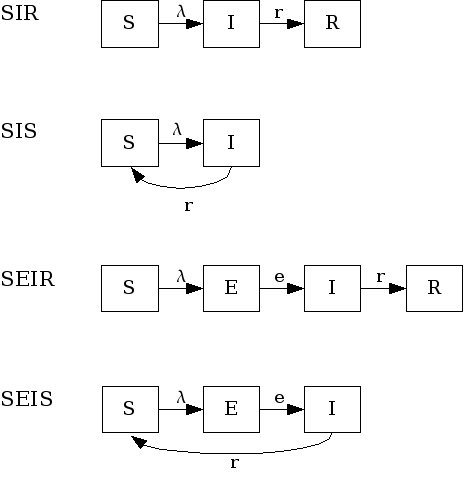
\includegraphics[scale=0.8]{SIRdiagram.png}
\caption{SIR-like models}
\label{fig:sir}
\end{center}
\end{figure}

Variations of this model consider that individuals do not acquire immunity after infection, thus returning to the susceptible pool (\textit{SIS} model). Another variation is the inclusion of a latent stage to hold individuals that are infected but not infectious to others yet (incubation period). These are the \textit{SEIR} (with immunity) and \textit{SEIS} (no immunity) models.

Next, we describe each one of these models in their deterministic and stochastic versions, as used by EpiGrass. 


\begin{description}
\item[SIR models]\index{Models!SIR}

Examples of diseases represented by SIR models are measles, chickenpox. Some diseases that do not confer lifelong immunity may be represented by this model if only short term dynamics is of interest. In the scale of a year, influenza and pertussis, for example, could be described using SIR. The SIR model is implemented in EpiGrass as a system of four difference equations. Besides the three equations describing the dynamics of $S$, $I$ and $R$, a fourth equation explicitly defines the number of new cases per time step, $L(t)$ (i.e., the incidence). In general, this quantity is embedded in the $I$ equation (prevalence), but it is important to keep track of the incidence if one wishes to compare prediction with notification data. 

\begin{align} \label{E:SIRmodel}
        L_{t+1} &= \beta S_t \frac{(I_t+\theta)^\alpha} {N_t+n_t}\nonumber \\
        I_{t+1} &= L_{t+1} + (1-r)I_t\nonumber\\
        S_{t+1} &= S_t + B - L_{t+1}\nonumber\\
        R_{t+1} &= N_t-(S_{t+1}+I_{t+1})
\end{align}

\begin{table}[h]
\caption{\small  Symbols used in the models and their meaning}
\begin{center}
\begin{tabular}{l l}
\hline\hline 
\textbf{Symbol}	&\textbf{Meaning}. \\ \hline	
$L_t$		& number of newly infected individuals at time t\\	
$E$		& number of exposed but not infectious individuals at time t\\
$I$		& number of infectious individuals at time t\\
$R$		& number of recovered individuals at time t\\
$\beta$		& contact rate ($t^{-1}$)\\
$\theta$	& number of infectious visitors\\
$\alpha$	& mixing parameter ($\alpha = 1$ means homogeneous mixing) \\
$n$		& number of visitors\\
$N$		& population ($S+E+I+R$)\\
$B$		& susceptible pool replenishment rate\\
$r$		& fraction of $I$ recovering from infection per unit of time ($[0,1]$)\\
$e$		& fraction of $E$ becoming infectious per unit of time ($[0,1]$)\\
$\delta$	& probability of acquiring immunity ($[0,1]$)\\
$w$		& probability of losing immunity($[0,1]$)\\ 
$p$		& probability of recovered individual acquiring infection, given exposure ($[0,1]$)\\\hline
\hline\hline
\label{Table:symbols}
\end{tabular}
\end{center}
\end{table} 

This model can be easily extended to include diseases without recovery, for example AIDS, the so called SI models. Basically, the recovery rate is set to 0.

\item[SIS models]\index{Models!SIS}
In the SIS model, individuals do not acquire immunity after the infection. They return directly to the susceptible class.

The only differences between $SIS$ and $SIR$ models is the absence of $R$ and the flow of recovered individuals to the susceptible stage: 

\begin{align} \label{E:SISmodel}
        L_{t+1} &= \beta S_t \frac{(I_t+\theta)^\alpha} {N_t+n_t} \nonumber\\
        I_{t+1} &= L_{t+1} + (1-r)I_t\nonumber\\
        S_{t+1} &= S_t + B - L_{t+1} + r I_{t+1}
\end{align}


\item[SEIR models]\index{Models!SEIR}
These models have an extra compartment for those individuals who have acquired the infection but are still not infectious to others. This is the latent period and it is often parameterized as the inverse of the incubation period. Note, however, that for many diseases, initiation of infectiousness does not necessarily coincides exactly with symptoms. In principle, any disease described by the SIR model can also be described by the SEIR model. The decision regarding the use of one or another depends on the magnitude of the latent period in relation to the time frame of other events in the simulation. The model has the form:

\begin{align} \label{E:SEIRmodel}
        L_{t+1} &= \beta S_t \frac{(I_t+\theta)^\alpha} {N_t+n_t}\nonumber \\
	E_{t+1} &= (1-e) E_t + L_{t+1}\nonumber\\
        I_{t+1} &= e E_t + (1-r)I_t\nonumber\\
        S_{t+1} &= S_t + B - L_{t+1}\nonumber\\
        R_{t+1} &= N_t-(S_{t+1}+I_{t+1}+E_{t+1})
\end{align}


 
\item[SEIS models]\index{Models!SEIS}

These are SIS models with the inclusion of the latent stage. 

\begin{align} \label{E:SEISmodel}
        L_{t+1} &= \beta S_t \frac{(I_t+\theta)^\alpha} {N_t+n_t}\nonumber \\
	E_{t+1} &= (1-e) E_t + L_{t+1}\nonumber\\
        I_{t+1} &= e E_t + (1-r)I_t\nonumber\\
        S_{t+1} &= S_t + B - L_{t+1} + r I_t
\end{align}

\end{description}

\subsubsection{SIpR-like models}

These are \textit{SIR} models with immunity intermediary between full (\textit{SIR}) and null (\textit{SIS}). 
Some possibilities arise here: 1) Infection confers full immunity to a fraction of the individuals and the remaining return to the susceptible class again, after infection. (\textit{SIpRpS}); 2) Infection provides only partial immunity and recovered individuals are partially susceptible to new infection (\textit{SIpR}); 3) Immunity is full right after infection but wanes with time (\textit{SIRS}). Each model is presented below. Figure \ref{fig:sipr} illustrates them diagrammatically.


\begin{figure}
\begin{center}
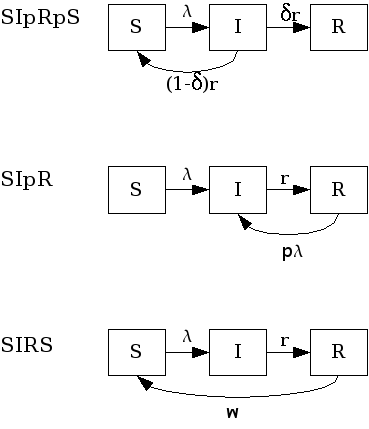
\includegraphics[scale=0.8]{SIpRdiagram.png}
\caption{SIpR-like models.}
\label{fig:sipr}
\end{center}
\end{figure}

Related models, that included the latent state $E$ are: \textit{SEIpRpS}, \textit{SEIpR}, \textit{SEIRS}.


\begin{description}
\item[SIpRpS model]\index{Models!SIpRpS}
This model assumes that a fraction $\delta$ of infectious individuals acquire full immunity while the remaining $(1-\delta)$ returns to the susceptible stage. The model is:

\begin{align} \label{E:SIpRpSmodel}
        L_{t+1} &= \beta S_t \frac{(I_t+\theta)^\alpha} {N_t+n_t}\nonumber \\
        I_{t+1} &= L_{t+1} + (1-r)I_t\nonumber\\
        S_{t+1} &= S_t + B - L_{t+1} + (1-\delta) r I_t\nonumber\\
        R_{t+1} &= N_t-(S_{t+1}+I_{t+1})
\end{align}


\item[SIpR model]
This model assumes that immunity is only partial and recovered individuals may acquire infection again (at a  lower rate $p \beta$, where $0\leq p \leq 1$). Two equations calculate the number of new infecteds. One, $L_S$  calculates the number of susceptibles that become infected at $t+1$. $L_R$  calculates the number of recovered that become infected at $t+1$. The latter are less susceptible to the disease and have (1-p)\% less chance of becoming infected, when compared to susceptibles. The model is:

\begin{align} \label{E:SIpRmodel}
        L_{S,t+1} &= \beta S_t \frac{(I_t+\theta)^\alpha} {N_t+n_t}\nonumber \\
	L_{R,t+1} &= p \beta R_t \frac{(I_t+\theta)^\alpha} {N_t+n_t}\nonumber\\ 
        I_{t+1} &= L_{S,t+1} + L_{R,t+1} + (1-r)I_t\nonumber\\
        S_{t+1} &= S_t + B - L_{S,t+1} \nonumber\\
        R_{t+1} &= N_t-(S_{t+1}+I_{t+1}) 
\end{align}


\item[SIRS model]\index{Models!SIRS}
Here, the immunity acquired by infection wanes with time. Pertussis and malaria are diseases with this characteristic.
\begin{align} \label{E:SIRSmodel}
        L_{S,t+1} &= \beta S_t \frac{(I_t+\theta)^\alpha} {N_t+n_t\nonumber} \\
	I_{t+1} &= L_{S,t+1} + L_{R,t+1} + (1-r)I_t\nonumber\\
        S_{t+1} &= S_t + B - L_{S,t+1} + w R_t\nonumber\\
        R_{t+1} &= N_t-(S_{t+1}+I_{t+1}) 
\end{align}


\end{description}


\subsubsection{SnInRn-like models}
These are models with more than one compartment for susceptibles, infected and recovered stages. They are used when infection involves more than one distinct populations. Vector borne diseases are classical examples where a SIR model is used to describe infection in humans and another SIR-like model is used to describe infection in the vector (and/or the reservoir(s)). Dengue fever and yellow fever are examples. Sexually transmitted diseases may also be modelled with SnInRn models if male and female populations are distinguished. These models are still not available in EpiGrass.


\subsection{Stochastic models}\index{Models!stochastic}

All models described so far are deterministic. EpiGrass allows simulation of stochastic processes. This is done by assuming that $L_{t+1}$ is a random variable with expected value given by the expressions found in the deterministic models. The user may choose the probability distribution for $L_{t+1}$ between Poisson or Negative Binomial to draw realizations of $L_{t+1}$:

$$
l_{t+1} \sim Poisson (L_{t+1})
$$

\begin{center}
or 
\end{center}

$$
l_{t+1} \sim NegBin (I_t, \frac{I_t}{I_t+L_{t+1}}) 
$$

The Poisson distribution assume independent events while the negative Binomial assume clustering of transmission events. 


\section{Network transportation models}\index{Models!transportation}


The transmission models describe the dynamics of infection in a well-mixed population. EpiGrass allows the user to model the movement of infectious individuals between well-mixed populations, thus simulating the spread of disease through space. EpiGrass represents geographical space as a network where cities or localities are nodes and transportation routes are edges. The term network refers to the framework of routes within a system of locations, identified as nodes or sites. An edge is a single link between two sites (a road, a railroad, an air route or a river/sea corridor).

Transportation networks, like many networks, are generally embodied as set of locations and a set of links representing connections between those locations. The arrangement and connectivity of a network is known as its \textit{topology}. Major types of topology are illustrated in \ref{fig:artgraphs}. Velocity and direction of disease spread depend on the topology and weight of the edges of the transport network and there are many properties of networks that may useful when analyzing the spread of diseases. EpiGrass calculates a set of these properties, described in \ref{cap:analysis}: 

In a transportation network, each edge (or link) is characterized by a variable $flow$ which states the number of passengers that travel through that link per unit time. EpiGrass uses this information to calculate the number of passengers arriving at each city, per time step. For example, consider node $N1$ in figure \ref{fig:simpnet}. At each time step, it receives 10 passengers form $N2$, 5 from $N5$, 1 from $N4$. Now suppose that, at this time step, 10\% of the population within each site is infectious ($I$ state), according to the epidemic model. Thus, a total of $10\% \times 10 + 10\% \times 5 + 10\% \times 1 = 1.6$ infectious individuals are visiting site $N1$. In the epidemic model embedded in $N1$, EpiGrass sets $n = 16$ and $\theta = 1.6$. 


\begin{figure}[ht]
\begin{center}
	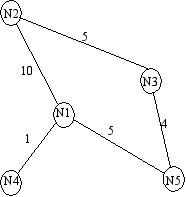
\includegraphics[scale=1.2]{simplenet.png}
\caption{A simple transportation network}
\label{fig:simpnet}
\end{center}
\end{figure}

%\subsection{Network topologies}

%Each transport network has a specific topology, that may depend on the scale of observation. Global transportation networks (as airlines) tend to a star configuration, with a few hubs. Terrestrial transportation tends to a mesh configuration. River networks tend to tree or linear topologies. 

%\begin{description}
%\item[Mesh network]
%\item[Star network]
%\item[Linear network]
%\item[Tree network]
%\item[Complete network]
%\item[Regular network]
%\end{description}

%\subsection{Network measures}

%With appropriate data, weights can be attributed to the edges. Figure shows a network with heterogeneous edges and nodes. The two dark nodes in the figure could represent important centers with large movement between them (thick lines). Peripheric localities, on the other hand, has lower connectance. Some measures presented here consider the weight of the edges, others not.


%\begin{description}
%\item[Distance matrix] The distance Matrix displays the number of edges between any
%        pair of nodes via the shortest path. 
%\item[Connectivity Matrix] The most basic measure of accessibility involves network connectivity
%        where a network is represented as a connectivity matrix(figure \ref{fig:cm}), which 
%        expresses the connectivity of each node with its adjacent nodes.    
%        The number of columns and rows in this matrix is equal to the number 
%        of nodes in the network and a value of 1 is given for each cell where 
%        this is a connected pair and a value of 0 for each cell where there 
%        is an unconnected pair. The summation of this matrix provides a very 
%        basic measure of accessibility, also known as the degree of a node.%
	
	
%\end{description}




%\section{The whole model}

%Combining the local epidemiological models to the dispersal network creates the full model implemented in %EpiGrass. 
%In the next section, you find an example of a whole model.


%\section{Example}



\chapter{Building and Installing}
\label{install} 
\lettrine{T}{his} chapter will walk through all aspects of EpiGrass installation. From obtaining, building and installing  the prerequisites to the installation of EpiGrass itself.

Most of the steps will be quite simple and similar since they will make use of standard tools for package installation on two very popular GNU/Linux distributions: Debian (and derivatives), and Gentoo. If you use a different distribution, you should check its documentation for package installation instructions.

If, on your distribution, a package is not available for the required version, you can try to obtain an updated version of the package at the web-sites provided. On the rare cases where pre-built packages are not available, instructions on how to build the software from source should also be available from its web-site.
\section{Required Packages}
\subsection{Python}
\begin{description}
\item[Web-site:] \url{http://www.python.org}
\item[Version required:] $\geq2.3$
\end{description}
Python is a simple but powerful object-orientated language. Its simplicity makes it easy to learn, but its power means that large and complex applications can be created. Its interpreted nature means that Python programmers are every productive because there is no edit/compile/link/run development cycle.

Python is probably installed automatically by your GNU/Linux distribution (it is on Gentoo). If not, it is best to use your distribution's standard tools for package installation. On Debian for example:
\begin{lstlisting}[frame=trBL, caption=Installation of Python in a Debian-based Gnu/Linux distribution. ,label=lst:pyinst]
$ apt-get install python
\end{lstlisting}

\subsection{Numeric Python}
\begin{description}
\item[Web-site:] \url{http://www.numpy.org}
\item[Version required:] $\geq23.0$
\end{description}
Numeric Python is a module for fast numeric computations in Python.

Example installations:
\begin{lstlisting}[frame=trBL, caption=Installing Numeric python on Gentoo GNU/Linux ,label=lst:instnumpyg]
$ emerge numeric
\end{lstlisting}
\begin{lstlisting}[frame=trBL, caption=Installing Numeric python on Debian GNU/Linux ,label=lst:instnumpyd]
$ apt-get install numeric
\end{lstlisting}

\subsection{Matplotlib}
\begin{description}
\item[Web-site:] \url{http://matplotlib.sourceforge.net}
\item[Version required:] $\geq0.70.0$
\end{description}
Matplotlib is a Module that provides plotting capabilities to Python.
\begin{lstlisting}[frame=trBL, caption=Installing Matplotlib on Gentoo GNU/Linux ,label=lst:instmplg]
$ emerge matplotlib
\end{lstlisting}
Before using \texttt{apt-get} to install matplotlib, add these lines to your  \texttt{/etc/apt/sources.list}:
\begin{lstlisting}[frame=trBL, caption=Adding specific sources to apt-get. ,label=]
deb http://anakonda.altervista.org/debian packages/
deb-src http://anakonda.altervista.org/debian sources/
\end{lstlisting}
\begin{lstlisting}[frame=trBL, caption=Installing Matplotlib on Debian GNU/Linux ,label=lst:instmpld]
$ apt-get update
$ apt-get install python-matplotlib python-matplotlib-doc
\end{lstlisting}


\subsection{Pygame}
\begin{description}
\item[Web-site:] \url{http://www.pygame.org}
\item[Version required:] $\geq1.6$
\end{description}
Pygame is a set of Python modules that wrap the excellent SDL library. Its the base of the EpiGrass OpenGL display.

Example installations:
\begin{lstlisting}[frame=trBL, caption=Installing Pygame python on Gentoo GNU/Linux ,label=lst:instpygameg]
$ emerge pygame
\end{lstlisting}
\begin{lstlisting}[frame=trBL, caption=Installing Pygame python on Debian GNU/Linux ,label=lst:instpygamed]
$ apt-get install pygame
\end{lstlisting}

\subsection{PyQt}
\begin{description}
\item[Web-site:] \url{http://www.riverbankcomputing.co.uk/pyqt/index.php}
\item[Version required:] $\geq3.13$
\end{description}
PyQt is a set of Python bindings for the Qt toolkit. PyQt combines all the advantages of Qt and Python. A programmer has all the power of Qt, but is able to exploit it with the simplicity of Python.

PyQt depends on the Qt libraries to run. This dependency will be taken care by the package installation tools of most distributions, which will automatically install the required version of Qt.

Example installations:
\begin{lstlisting}[frame=trBL, caption=Installing PyQt python on Gentoo GNU/Linux ,label=lst:instpyqtg]
$ emerge pyqt
\end{lstlisting}
\begin{lstlisting}[frame=trBL, caption=Installing PyQt python on Debian GNU/Linux ,label=lst:instpyqtd]
$ apt-get install python2.3-qt3
\end{lstlisting}
\subsection{MySQL}
\begin{description}
\item[Web-site:] \url{http://www.mysql.com}
\item[Version required:] $\geq4.0$
\end{description}
MySQL is a fast, multi-threaded, multi-user SQL database server. If you have a MySQL server available in your LAN, you may skip this step after making sure you have permission to access and use it to store your data.

Example installations:
\begin{lstlisting}[frame=trBL, caption=Installing MySQL on Gentoo GNU/Linux ,label=lst:instmysqlg]
$ emerge mysql
\end{lstlisting}
\begin{lstlisting}[frame=trBL, caption=Installing MySQL on Debian GNU/Linux ,label=lst:instmysqld]
$ apt-get install mysql-server
$ apt-get install mysql-client
\end{lstlisting}

\paragraph*{Post-install configuration:}
MySQL requires a few extra configuration steps that must be completed after the installation described above. These steps must be performed by the root user.
\begin{lstlisting}[frame=trBL, caption=Post-install configuration of mysql on Gentoo ,label=lst:mysqlconfg]
$ /etc/init.d/mysql start
$ mysql_install_db
$ mysqladmin -u root password new-password
$ rc-update add mysql default
\end{lstlisting}
In the mysqladmin line, replace new-password with a password of your own. 

\begin{lstlisting}[frame=trBL, caption=Post-install configuration of mysql on Debian ,label=lst:mysqlconfd]
$ mysql_install_db
$ safe_mysqld &
$ /etc/init.d/mysql start
$ mysqladmin -u root password new-password
\end{lstlisting}

\subsection{MySQL-python}
\begin{description}
\item[Web-site:] \url{http://sourceforge.net/projects/mysql-python/}
\item[Version required:] $\geq0.9.2$
\end{description}
This package is a MySQL module for Python.

Example installations:
\begin{lstlisting}[frame=trBL, caption=Installing MySQL-python on Gentoo GNU/Linux ,label=lst:instmysqlpyg]
$ emerge mysql-python
\end{lstlisting}
\begin{lstlisting}[frame=trBL, caption=Installing MySQL-python  on Debian GNU/Linux ,label=lst:instmysqlpyd]
$ apt-get install python2.3-mysqldb
\end{lstlisting}
\subsection{R}
\begin{description}
\item[Web-site:] \url{http://www.r-project.org}
\item[Version required:] $\geq2.0$
\end{description}
Example installations:
\begin{lstlisting}[frame=trBL, caption=Installing R on Gentoo GNU/Linux ,label=lst:instRg]
$ emerge R
\end{lstlisting}
\begin{lstlisting}[frame=trBL, caption=Installing R on Debian GNU/Linux ,label=lst:instRd]
$ apt-get install r-base
\end{lstlisting}
\paragraph*{Post-install configuration:}
You have to install a few packages from within R afterward.
\begin{lstlisting}[frame=trBL, caption=Installing aditional packages from within R ,label=lst:instRpkgs]
> install.packages('RMySQL')
> install.packages('DBI')
> install.packages('lattice')
\end{lstlisting}

\subsection{RPy}
\begin{description}
\item[Web-site:] \url{http://rpy.sourceforge.net/}
\item[Version required:] $\geq0.4.0$
\end{description}
RPy is a very simple, yet robust, Python interface to the R Programming Language. It can manage all kinds of R objects and can execute arbitrary R functions (including the graphic functions). 
Example installations:
\begin{lstlisting}[frame=trBL, caption=Installing RPy on Gentoo GNU/Linux ,label=lst:instRPyg]
$ emerge rpy
\end{lstlisting}
If the \texttt{rpy} package on Gentoo is masked\footnote{Meaning that it can't be installed normally.}, use the method described for installing on Debian, below. 

On Debian download the RPy source tarball, unpack it, \texttt{cd} to the directory to which you unpacked it and type:
\begin{lstlisting}[frame=trBL, caption=Installing RPy on Debian GNU/Linux ,label=lst:instRPyd]
$ python setup.py install
\end{lstlisting}
RPy depends on R having been compiled with the option \texttt{--enable-R-shlib}. This is the default on Gentoo. If this installation fails on your system, you may have to get the latest version from rpy from its website and install from source by following these steps:
\begin{enumerate}
\item First of all, you \textbf{must} check that you have built R with the configure
    option '--enable-R-shlib', in order to make R as a shared library.  If
    not, the following steps should be enough:
\begin{lstlisting}[frame=trBL, caption=Building R from source ,label=lst:rfs]
 <go to the R source directory>
$ make distclean
$ ./configure --enable-R-shlib
$ make
$ sudo make install
\end{lstlisting}
 


\item Then, configure the path to the R library. For this, make a link to RHOME/bin/libR.so in /usr/local/lib or /usr/lib, then run \texttt{ldconfig},  (substitute RHOME with the path where R is installed, usually
    \/usr\/local\/lib\/R):
\begin{lstlisting}[basicstyle=\footnotesize,frame=trBL, caption= ,label=]
$ sudo ln -s /usr/local/lib/R/lib/libR.so /usr/lib/libR.so
\end{lstlisting}

\item Ensure that you have the necessary header files for the version of R you are 
    compiling against.  You can check the version of R by running:
\begin{lstlisting}[frame=trBL, caption= ,label=]
$ R --version
R 2.0.1 (2004-11-15).
Copyright (C) 2004 R Development Core Team

R is free software and comes with
ABSOLUTELY NO WARRANTY.
You are welcome to redistribute it under 
the terms of the GNU General Public License.  
For more information about these matters,
see http://www.gnu.org/copyleft/gpl.html.
\end{lstlisting}


    There should be a subdirectory of the Rpy package with the name
\texttt{R-<version>}.For the example above, \texttt{R-2.0.1}

    If the correct version directory does not exist, you may have to go back to a version of \texttt{R} supported by rpy.


\item Now, just type:
\begin{lstlisting}[frame=trBL, caption= ,label=]
$ python setup.py install
\end{lstlisting}
       

    and that's all!

\end{enumerate}



\subsection{Grass GIS}
\begin{description}
\item[Web-site:] \url{http://grass.itc.it/}
\item[Version required:] $\geq5.0.3$
\end{description}
\begin{lstlisting}[frame=trBL, caption=Installing GRASS on Gentoo GNU/Linux ,label=lst:instgrassg]
$ emerge grass
\end{lstlisting}

\begin{lstlisting}[frame=trBL, caption=Installing GRASS on Debian GNU/Linux ,label=lst:instgrassd]
$ apt-get install grass
\end{lstlisting}

\subsection{\LaTeX}
\begin{description}
\item[Web-site:] \url{http://www.tug.org/teTeX/}
\item[Version required:] $\geq2.0$
\end{description}
EpiGrass uses \LaTeX  or PDF\LaTeX  to generate a report with a summary analysis of your network and simulation model. Thus, it is necessary to have the Tetex package installed.
\begin{lstlisting}[frame=trBL, caption=Installing \LaTeX and PDF\LaTeX on Gentoo GNU/Linux ,label=lst:insttexg]
$ emerge tetex
\end{lstlisting}

\begin{lstlisting}[frame=trBL, caption=Installing \LaTeX and PDF\LaTeX on Debian GNU/Linux ,label=lst:insttexd]
$ apt-get install tetex-base
\end{lstlisting}

\section{Installing EpiGrass}
If you got through all the steps above, it will be an easy task to install EpiGrass:
\begin{lstlisting}[frame=trBL, caption=Intalling EpiGrass ,label=lst:instepg]
$ python setup.py install
\end{lstlisting}

We have written an ebuild for installing epigrass on Gentoo. If it is unmasked at the time you decide to install epigrass, you don't need to worry about the dependencies above and only need to type the following command:
\begin{lstlisting}[frame=trBL, caption=Installing EpiGrass on Gentoo GNU/Linux ,label=lst:instepgg]
$ emerge epigrass
\end{lstlisting}  % install
\chapter{Using Epigrass} 
\label{ch:usingepg}

\lettrine{T}{o} simulate an epidemic process in EpiGrass, the user needs to have in hand three files: Two files containing the site and edge data and a third file which is a script that defines what it is to be done. Here we go through each one of them in detail. As the last part of this chapter, is a step-by step guide the Graphical User Interface (GUI).

\section{Data}

\subsection{Site data file}
See below an example of the content of a site file for a network of 10 cities. Each line corresponds to a site (except the first line which is the title). For each site, it is declared, in this order: its \textit{spatial location} in the form of a pair of coordinates ([X,Y]); a site $name$ to be used in the output; the site's population; the site geocode (an arbitrary unique number which is used internally by EpiGrass).

\begin{lstlisting}[frame=trBL, caption= ,label=]
X,Y,City,Pop,Geocode
1,4,"N1",1000000,1
2,4,"N2",100000,2
3,4,"N3",1000,3
4,4,"N4",1000,4
5,4,"N5",1000,5
1,3,"N6",100000,6
2,3,"N7",1000,7
3,3,"N8",100000,8
4,3,"N9",100000,9
5,3,"N10",1000,10
1,2,"N11",1000,11
\end{lstlisting}

In this example, the first site is located at $[X,Y]=[1,4]$, it is named N1, its population is 1000000 and its geocode is 1. This is minimum configuration of a site data file and it must contains this information in exactly this order. 

In some situations, the user may want to add other attributes to the sites (different transmission parameters, or vaccine coverage or initial conditions for simulations). This information is provided by adding new columns to the minimum file. For example, if one wishes to add information on the vaccine coverage in cities N1 to N10 ($vac$) as well as information about average temperature (which hypothetically affects the transmission of the disease), the file becomes:

\begin{lstlisting}[frame=trBL, caption= ,label=]
X,Y,City,Pop,Geocode,Vac,Temp
1,4,N1,1000000,1,0.9,32
2,4,N2,100000,2,0.88,29
3,4,N3,1000,3,0.7,25
4,4,N4,1000,4,0.2,34
5,4,N5,1000,5,0,26
1,3,N6,100000,6,0,27
2,3,N7,1000,7,0,31
3,3,N8,100000,8,0,30
4,3,N9,100000,9,0,24
5,3,N10,1000,10,0,31
\end{lstlisting}

During the simulation, each site object receives these informations and store them in appropriate variables that can be used later during model specification. Population is stored in the variable $N$; while the extra columns (those beyond the geocode) are stored in a tuple named \textit{values}. For example, for the city $N1$, we have $N = 1000000$ and $values=[0.9,32]$. During model specification, we may use $N$ to indicate the population size and/or we can use $values[0]$ to indicate the level of vaccination of that city and $values[1]$ to indicate the temperature. 

It is up to the user, to know what means the elements of the tuple $values$. Note that the first element of the tuple has index 0,the second one has index 1 and so on.

When using real data, one may wish to use actual geocodes and coordinates. For example, for a network of Brazilian cities, one may build the following file:


\begin{lstlisting}[frame=trBL, caption= ,label=]
latitude,longitude,local,pop,geocode
-16:19:41,-48:57:10,ANAPOLIS,280164,520110805
-10:54:32,-37:04:03,ARACAJU,461534,280030805
-21:12:27,-50:26:24,ARACATUBA,164449,350280405
-18:38:44,-48:11:36,ARAGUARI,92748,310350405
-21:13:17,-43:46:12,BARBACENA,103669,310560805
-22:32:53,-44:10:30,BARRA_MANSA,165134,330040705
-20:33:11,-48:34:11,BARRETOS,98860,350550005
-26:54:55,-49:04:15,BLUMENAU,241943,420240405
-22:57:09,-46:32:30,B.PAULISTA,111091,350760505
\end{lstlisting}



In this file, the coordinates are the actual geographical latitude and longitude coordinates. This information is important when using EpiGrass integrated with Grass GIS. The geocode is also the official geocode of these localities. Despite the cumbersome size of the number, it may be worth using it because demographic official databases are often linked by this number.



\subsection{Edge data file}

The edge data file contains all the direct links between sites. Each line in the file (except the first) corresponds to an edge. For each edge (or link) one must specify (in this order): the \textit{names of the sites} connected by that edge; the \textit{number of individuals traveling from source to destination}; the \textit{number of individuals travelling from destination to source} per time step; the \textit{distance or length} of the edge. At last, the file must contain, in the fifth and sixth columns, the \textit{geocodes of the source and destination sites}. This is very important as graph is built internally connecting sites through edges and this is done based on geocode info. 

\vspace{1cm}
\textbf{IMPORTANT: It is required that the order of columns is kept the same}
\vspace{1cm}

See below the list of the 8 edges connecting the sites $N1$ to $N10$. Let's look the first one, as an example. It links $N1$ to $N2$. Through this link passes 11 individuals backwards and forwards per time step (a day, for example). This edge has length 1 (remember that $N1$ is at [X,Y]=[1,1] and $N2$ is at [X,Y]=[1,2], so the distance between them is 1). The last two columns show the geocode of $N1$ (geocode 1) and the geocode of $N2$ (geocode 2).

\begin{lstlisting}[frame=trBL, caption= ,label=]
Source,Dest,flowSD,flowDS,Distance,geoSource,geoDest
N1,N2,11,11,1,1,2
N2,N4,0.02,0.02,1,3,4
N3,N8,1.01,1.01,1,3,8
N4,N9,1.01,1.01,1,4,9
N5,N10,0.02,0.02,1,5,10
N6,N5,1.01,1.01,1,7,8
N7,N10,1.01,1.01,1,7,8
N9,N10,1.01,1.01,1,9,10
\end{lstlisting}

Note that it doesn't matter which site is considered a Source and which one is considered a Destination. I.e., if there is a link between $A$ and $B$, one may either named $A$ as source and $B$ as destination, or the other way around.

If the edge represents a road or a river, one may use the actual metric distance as length. If the edge links arbitrary localities, one may opt to use euclidean distance, calculated from the x and y coordinates (using Pitagoras theorem). 



\section{Specifying a model: the script}

Once the user has specified the two data files, the next step is to define the model to be executed. This is done in the .EPG script file. The .EPG script is a text file and can be edited with any editor (not word processor). This script must be prepared with care. 

The best way to write down your own .EPG is to edit an already existing .epg file. So, open \textbf{EpiGrass}, choose an .epg file and click on the \textbf{Edit} button. Your favorite editor will open and you can start editing. Don't forget to save it as a new file in your working directory. Of course, there is an infinite number of possibilities regarding the elaboration of the script. It all depends on the goals of the user. 

For the beginner, we suggest him/her to take a look at the .epg files in the demo directory. They are all commented and may help the user in getting used with Epigrass language and capabilities.

Some hints to be successful when editing your .EPG:

\begin{itemize}
\item  All comments in the script are preceeded by the symbol \#. These comments may be edited by the user as he/she wishes and new lines may be added at will. Don't forget, however, to place the symbol \# in every line corresponding to a comment.
\item The script is divided into a few parts. These parts have capital letter titles within brackets. Don't touch them!
\item Don't remove any line that is \textit{not} a comment. See below how to appropriately edit these command lines. 
\end{itemize}

Let's take a look now at each part of a script (this is the script.epg demo file):

\subsection{PART 1: THE WORLD}

The first section of the script is titled: THE WORLD. An example of its content is shown:
 
\begin{lstlisting}[basicstyle=\footnotesize,language=Python, frame=trBL, caption= ,label=]
#=========================================================#
[THE WORLD]
#=========================================================#

location = BRASIL
vector layer = Limite_politico_administrativo
sites = sitios2.csv
edges = edgesout.csv
\end{lstlisting}

where 

\begin{description}
\item[location:] indicates the GRASS location where maps (raster and vector maps) for the region are stored (required only if GRASS location exists. If not, leave it blank: $location =$ ). 
\item[vector layer:] Name of the vector layer, in the GRASS location, to be used as background to the network visualizer. 
\item[sites:] this is the name of the .CSV file containing the list of sites and their attributes.
\item[edges:] this is the name of the .CSV file containing the list of edges and their attributes.
\end{description}

\subsection{PART 2: EPIDEMIOLOGICAL MODEL}

This is the main part of the script. It defines the epidemiological model to be run.
The script reads:

\begin{lstlisting}[basicstyle=\footnotesize,language=Python, frame=trBL, caption= ,label=]
#=========================================================#
[EPIDEMIOLOGICAL MODEL]
#=========================================================#
#model types available: SIS, SIS_s ,SIR, SIR_s, SEIS, SEIS_s, SEIR, SEIR_s, 
# SIpRpS, SIpRpS_s,SIpR,SIpR_s(see documentation for description)
modtype = SIR

\end{lstlisting}

Here, the type of epidemiological model is defined, in this case is a deterministic SIR model. EpiGrass has some built-in models:


\begin{center}
\begin{tabular}{l l l}
\hline 
\textbf{Model}	&\textbf{Detemrinistic} &\textbf{Deterministic}. \\ \hline	
Susceptible-Infected-Recovered  & $SIR$	& $SIR_s$\\
Susceptible-Exposed-Infected-Recovered & $SEIR$	& $SEIR_s$\\
Susceptible-Infected-Susceptible & $SIS$  &  $SIS_s$\\
Susceptible-Exposed-Infected-Susceptible & $SEIS$ & $SEIS_s$\\
SIR with fraction with full immunity & $SIpRpS$ & $SIpRpS_s$\\
SEIR with fraction with full immunity & $SEIpRpS$ & $SEIpRpS_s$\\
SIR with partial immunity for all & $SIpR$ & $SIpR_s$\\
SEIR with partial immunity for all & $SEIpR$ & $SEIpR_s$\\
SIR with immunity wane & $SIRS$ & $SIRS_s$\\
\hline
\end{tabular}
\end{center}

A description of these models can be found in section \ref{cap:modeling}. The stochastic models use Poisson distribution as default for the the number of new cases ($L_{t+1}$). Following the script, we find:

\begin{lstlisting}[basicstyle=\footnotesize,language=Python, frame=trBL, caption= Defining model parameter and initial values ,label=lst:pars]
#==============================================================#
[MODEL PARAMETERS]
#==============================================================#

#  They can be specified as constants or as functions of global or 
#  site-specific variables. these site-specific variables, are provided
#  in the sites file. All the numbers given after the geocode (4th column)
#  are collected into the values tuple.
# Examples:
# beta = 0.001
# beta=values[0] #assigns the first element of values to beta 
# beta=0.001*values[1]

beta = 0.4   #transmission coefficient (contact rate * transmissibility)
alpha = 1  # clumping parameter
e = 1   # inverse of incubation period
r = 0.1   # inverse of infectious period
delta = 1  # probability of acquiring full immunity [0,1]
B = 0           # Birth rate
w = 0           # probability of immunity waning [0,1]
p = 0           # 

\end{lstlisting}

These are the model parameters, as described in \ref{Table:symbols}. Not all parameters are necessary for all models. For example, $e$ is only required for SEIR-like models. Don't
remove the line, however because that will cause an error. We recommend that, if the parameter is not necessary, just add a comment after it as a reminder that it is not being used by the model.

In some cases, one may wish to assign site-specific parameters. For example, transmission rate may be different between localities that are very distant and are exposed to different climate. In this case site specific variables can be added as new columns to the site file. All columns after the geocode are packed into a tuple named \textit{values} and can be referenced as shown in listing \ref{lst:pars}. I.e., the first element of the tuple is values[0], the second element is values[1], the third element is values[2] and so on.

The next part of the script, the initial conditions are defined. Here, the number of individuals in each epidemiological state, at the start of the simulation, is specified.The script reads:

\begin{lstlisting}[basicstyle=\footnotesize,language=Python, frame=trBL, caption= ,label=]
[INITIAL CONDITIONS]

# Here, the number of individuals in each epidemiological
# state (SEI) is specified. They can be specified in absolute
# or relative numbers.
# N is the population size of each site.
# The rule defined here will be applied equally to all sites.
# For site-specific definitions, use EVENTS (below)
# Examples:
#	S,E,I = 0.8*N, 10, 0.5*N
#	S,E,I = 0.5*N, 0.01*N, 0.05*N
#	S,E,I = N-1, 1, 0
S = N
E = 0
I = 0
\end{lstlisting}

Here, $N$ is the total population in a site (as in the datafile for sites). In this example, we set all localities to the same initial conditions (all individuals susceptible) and use an event (see below) to introduce an infectious individual in a locality. The number of recovered individuals is implicit, as $R = N-(S+E+I)$

Another possibility is to define initial conditions that are different for each site. For this, the data must be available as extra columns in the site datafile and these columns are referrenced to using the \textit{values} tuple explained above.

The next step is to define events that will occur during the simulation. These events may be epidemiological (arrival of an infected, for example) or a public health action (vaccination campaign, for example):

\begin{lstlisting}[basicstyle=\footnotesize,language=Python, frame=trBL, caption=Defining epidemic events ,label=lst:event]
[EPIDEMIC EVENTS]

# Specify isolated events.
# Localities where the events are to take place should be Identified by a numeric code 
# to come after population size on the sites data file.
# Seed : [('locality1's geocode', n),('locality2's geocode', n)]. 
# N infected cases will be added to locality at time 0.
# Vaccinate: [('locality1's geocode', time, coverage),('locality2's geocode', time, coverage)] 
# Quarantine: [(locality1's geocode,time,duration), (locality2's geocode,time,duration)]
seed = [(230440005,1)] #Fortaleza
Vaccinate = [(355030800, 31, 0.9)] #Sao Paulo
Quarantine = [(355030800,20)]
\end{lstlisting}

The events currently implemented are:
\begin{description}
\item{seed} One infected individual is introduced into a site. The notation for a single event is:
$$seed = [(geocode,time step)]$$
For example, $seed = [(2,1)]$ programs the arrival of an infected individual at site geocode 2, at time 1. 
For several events, the notation is:
$$seed = [(geocode1,time step1),(geocode2,time step2),(geocode3,time step3)]$$
There is no limit to the number of events that can be included in this list.
\item{Vaccinate} Implements a campaign that vaccinates a fraction of the population in a site, at a pre-defined time-step. For a single event, the notation is:
$$[(geocode1, time, coverage)]$$
where the first element is the geocode of the city, the second element is the time when the campaign is implemented and the third element is the coverage. For example, the event $[(2,10,0.7)]$ means that city 2, at time 10, has 70\% of its population vaccinated. Mathematically, it means (in the model), the removal of individuals from the susceptible to the recovered stage.
For several events, we may have simultaneous vaccinations at two sites:
$$Vaccinate = [(1, 31, 0.9),(2,31,0.9)]$$ 
or subsequent campaigns in the same site:
$$Vaccinate = [(1, 31, 0.2),(1,61,0.3)]$$ 
\item{Quarantine} Prevents any individual from leaving a site, starting at $t$. The notation is:
$$Quarantine = [(geocode1,t),(geocode2,t)]$$
As an example, a quarantine in locality 2, that starts at day 10 is noted:
$Quarantine = [(2,10)]$
\end{description}

\subsection{PART 3: TRANSPORTATION MODEL}

Here, there are two options regarding the movement of infected individuals from site to site (through the edges). If $stochastic = 0$, the process is simulated deterministically. The number of infected passengers commuting through an edge is a fraction $p$ of the infected population that is traveling. $p$ is calculated as $\frac{total passengers}{total population}$ . 

If $stochastic = 1$, the number of passengers is sampled from a Poisson distribution with parameter given by the expected number of travelling infectives (calculated as above).  

\begin{lstlisting}[basicstyle=\footnotesize,language=Python, frame=trBL, caption= ,label=]
#=========================================================#
[TRANSPORTATION MODEL]
#=========================================================#
# If doTransp = 1 the transportation dynamics will be 
# included. Use 0 here only for debugging purposes.
doTransp = 1

# Mechanism can be stochatic (1) or deterministic(0). 
stochastic = 1

\end{lstlisting}

That ends the definition of the model. 
\subsection{SIMULATION AND OUTPUT}
Now it is time to define some final operational variables for the simulation:

\begin{lstlisting}[basicstyle=\footnotesize,language=Python, frame=trBL, caption= ,label=]
#=========================================================#
[SIMULATION AND OUTPUT]
#=========================================================#

# Number of steps
steps = 200

# Output dir
outdir = ~/data

# Output file
outfile = simul.dat

# Database Output
# MySQLout can be 0 (no database output) or 1
MySQLout = 1 

# Graphical outputs
draw map = 1

# Report Generation
# The variable report can take the following values:
# 0 - No report is generated.
# 1 - A network analysis report is generated in PDF Format.
# 2 - An epidemiological report is generated in PDF Format.
# 3 - A full report is generated in PDF Format.
# siteRep is a list with site geocodes. For each site in this list, a detailed report is apended to the main report.
report = 0
siteRep = [230440005,355030800]

#Batch Run
#  list other scripts to be run in after this one. don't forget the extension .epg
#  model scripts must be in the same directory as this file or provide full path.
#  Example: Batch = ['model2.epg','model3.epg','/home/jose/model4.epg']
Batch = []
\end{lstlisting}

where
\begin{description}
\item[step] Number of time steps for the simulation.
\item[outdir] Directory for data output (currently not in use)
\item[outfile] .csv filename that can be imported into R as a dataframe. This .csv file contains the simulated timeseries for all nodes.
\item[MySQLout] Use MySQLout $= 1$ if simulated time series are to be stored in MySQL database. Time series of $L$,$S$,$E$,and $I$, from simulations, are stored in a MySQL database named \emph{epigrass}. The results of each individual simulation is stored in a different table named after the model's script name, the date and time the simulation has been run. For instance, suppose you run a simulation of a model stored in a file named \texttt{script.epg}, then at the end of the simulation, a new table in the epigrass database will be created with the following name: \texttt{script\_Wed\_Jan\_26\_154411\_2005}. Thus, the results of multiple runs from the same model get stored independently.
\item[draw map]
\item[report]Three types of report are currently available: $Report = 1$ returns a set of descriptors of the network, described in \ref{cap:analysis}; $Report = 2$ returns a set of basic epidemiological measures and plots of the time series; $Report = 3$ is $Report 1 + Report 2$. Report Generation is an optional, though recommended, step done at the end of the simulation. For the report, descriptive statistics are generated for the network. These have to do with network topology and properties. Additional sections can be added to the report with basic statistical analyses of the output of pre-selected nodes, listed  in the $siteRep$ variable at the script.
\item[siteRep=[]] List of nodes for which network and epidemiological measures are to be calculated and included in the report.
\item[Batch=[]] script files included in this list are executed after the currently file is finished.
\end{description}
\section{User defined models}
In future releases Epigrass will allow the user to define epidemiological models to be included into the sites.


\section{Using Epigrass for specific tasks}

Here we describe some things you could do with epigrass and some specific hints:

\subsection{Describing a network}
A user wants to obtain the topological properties of a network. Reasons for this could be: 1) learn how to interpret these measures, 2) describe a air transportation or a road transportation network. To do that, you need:

\begin{description}
\item[Set steps = 1]. If no model of disease is needed, then most of the .epg script can be ignored. Don't remove anything, however, from the script.  Note that Epigrass requires a model in order to work properly, even if the user does not want it. One solution to reduce the run time, in this case, is to set \textbf{steps} to 1 (steps = number of steps in the simulation).
\item[Set MySQLout = 0]. Network measures are not sent to database.
\item[Set report = 1]. Report 1 calculates network measures and save them in a .pdf file.
\item[Especify siteRep]. If siteRep = [], only global network measures are included in the report. If site-specific measures are needed, include their geocodes in the list siteRep. For example, to calculate site stats for all nodes, mesh1.epg has:
\begin{verbatim}
report = 1
siteRep = [1,2,3,4,5,6,7,8,9,10,11,12,13,14,15,16,17,18,19,20]
\end{verbatim}
\end{description}

Script mesh1.epg is configured this way. Run it and take a look at the report. 


\subsection{Comparing networks}
A user wants to compare the properties of a set of networks. Reasons for this could be: 1) learn how to interpret these measures, 2) describe/compare a air transportation to a road transportation network, 3) analyse how network topology changes by adding/removing specific nodes or edges.

If there are four graphs, then four .epg files must be created. They all must set $report=1$ and $siteRep$ to the desired specification (as above). Each file must be executed and each one will provide a report. 

To quick thinks a little bit, the script allows the user to choose one of the files as a master file. In the option $BatchRun$, one may list the other scripts to be run after this one. They all must be in the same directory as the master file (or you may provide full path).

For example, suppose you want to compare the topologies of the four networks displayed in \ref{fig:artgraphs}.
 
 \begin{center}
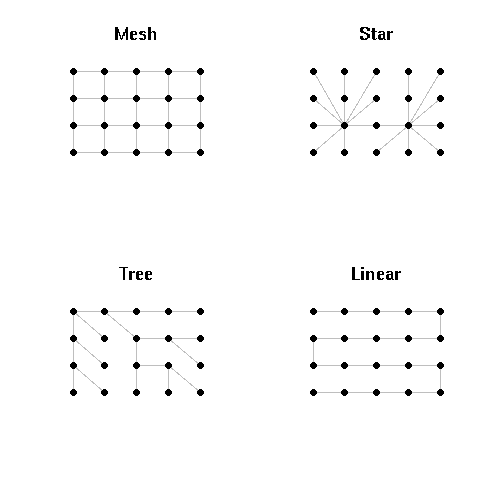
\includegraphics[scale=0.5]{artgraphs.png}
%\caption{SIR-like models}
\label{fig:artgraphs}
\end{center}

 
We created four files (mesh2.epg, star2.epg, lin2.epg, tree2.epg) and used one of them as master (mesh2.epg). The four files are exactly the same, except for the name of the edge file and the \textbf{Batch} specification. I.e., in mesh2.epg we specify:
\begin{verbatim}
Batch = ['star2.epg','lin2.epg','tree2.epg']
\end{verbatim}
Now, mesh2.epg is run. One report will be delivered for each script (In future version of Epigrass, a more integrated result is planned). From the reports, we get network measures for the four graphs. These network measures are explained in chapter \ref{cap:analysis}). 


\subsection{Simulate disease spread from a single site}
The user specifies a network (let's say, a tree network) and wishes to simulate disease spread in this network. The graph is disease-free at time 0. At time 1, an infected person arrives at site $N1$. No control measures are introduced. The model chosen is SipRpS. 
The script file tree3.epg was built following these guidelines:
\begin{description}
\item[Initial conditions] All individuals are initially susceptible, i.e.,  $S=N$.  
\item[Epidemic events] An infected individual arrives at time 1 in N1.
\item[steps=200] This may be increased or reduced, depending on the parameters.
\item[Report = 2]. Report 2 returns only the epidemiological results.
\item[Specify siteRep]. If site-specific measures are needed, include their geocodes in the list siteRep. For example, to calculate site stats for three nodes, tree3.epg has:
\begin{verbatim}
report = 2
siteRep = [1,12,14]
\end{verbatim}
Run this script and take a look at the report. A sugestion: change the script and seed the disease in a more central node. See how this affect the velocity of disease propagation.
\end{description}

\subsection{Simulating vaccination campaigns}
Vaccination may be simulated in different ways, using the section Epidemic Events in the script. These are some examples:
\begin{description}
\item[A single, local campaign].  In site N1, exactly at time 10, with coverage 0.5
\begin{verbatim}
Vaccinate = [(1,10,0.5)]
\end{verbatim}
\item[Simultaneous campaigns in three sites].  In sites N1, N4 and N6, exactly at time 10, with coverage 0.5
\begin{verbatim}
Vaccinate = [(1,10,0.5),(4,10,0.5),(6,10,0.5)]
\end{verbatim}
\item[Campaign with a time span].  In site N1, a campaign that occurs from day 10 to day 15, with daily coverage of 0.1.
\begin{verbatim}
Vaccinate = [(1,10,0.1),(1,11,0.1),(1,12,0.1),(1,13,0.1),
(1,14,0.1),(1,15,0.1)]
\end{verbatim}
\end{description}


\subsection{Simulating quarantines}
Quarantines are simulated similarly to vaccinations, but once they are initiated, they last until the end of the simulation:
\begin{description}
\item[Quarantine in a single place].  In site N1, starting at time 10, with coverage 0.2
\begin{verbatim}
Quarantine = [(1,10,0.2)]
\end{verbatim}
\item[Quarantine in two places].  In sites N1 and N3, at times 10 and 12, respectively, with coverage 0.5
\begin{verbatim}
Quarantine = [(1,10,0.5),(3,12,0.5)]
\end{verbatim}
\item[Quarantine with a time span].  In site N1, a quarantine that starts at day 10 and ends at time 30, with daily coverage of 0.75.
\begin{verbatim}
Quarantine = [(1,10,0.75),(1,30,0)]
\end{verbatim}
\end{description}

\subsection{Comparing strategies}
One goal of modeling diseases is to compare alternative control measures in terms of number of cases prevented. A set of scripts may be prepared to compare six alternative strategies for controlling the spread of an epidemic in the star graph, that was initiated at time 4 in site N1. For example:
\begin{description}
\item[Strategy vac1]  Vaccinate site $N1$, at time $7$, with coverage $0.8$ .
\item[Strategy vac2]  Vaccinate sites $N1$, $N12$ and $N14$, at time $7$, with coverage $0.8$. $N12$ and $N14$ are central nodes of the star network and are natural candidates for vaccination.
\item[Strategy mixed] Strategy vac1 $+$ quarantine in sites $N12$ and $N14$, coverage of $0.7$.
\item[Strategy quar] Quarantine in sites $N1$, $N12$ and $N14$, coverage of $0.7$.
\end{description}


\section{The Graphical User Interface(GUI)}
Epigrass comes with a simple but effective GUI(figure \ref{fig:gui}), that allows the user to control some aspects of the run-time behavior of the system. The Gui can be invoked by typing \texttt{epigrass} in prompt of a console. We suggest the user to start EpiGrass from the same directory where his/her model definition is located (.csv and .epg files).

All the information that is entered via the GUI gets  stored in a hidden file called \texttt{.epigrassrc} stored in the home folder of the user. Every time the GUI is invoked, the data stored in the \texttt{.epigrassrc} file is used to fill the forms in the GUI. The gui is designed as a tabbed notebook with four tabs (Run Options, Settings, Utilities, and Visualization).

At the bottom of the Gui there are three buttons \texttt{Help}, \texttt{Start} and \texttt{Exit}. Their functions will be explained below. Immediately above the \texttt{Run} and \texttt{Exit} buttons, there is a small numeric display that will display the simulation progress after it has been started.
\begin{figure}
	\centering
%	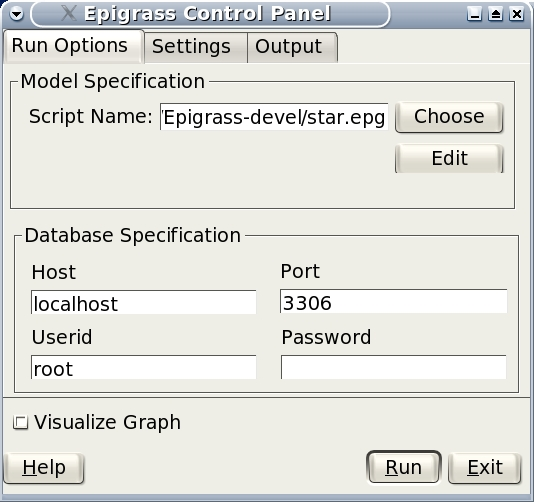
\includegraphics[scale=0.7]{gui.jpg}
% gui.jpg: 72dpi, width=18.84cm, height=17.71cm, bb=0 0 534 502
	\caption{First tab of the EpiGrass GUI.}
	\label{fig:gui}
\end{figure}

\subsection{Run Options}
The first tab of the GUI(figure \ref{fig:gui}), contains a number of variables that, with the exception of the model script filename, should remain the same for most simulations you are going to run.

On the top of the first tab is a text box to enter the file name of the model script (\texttt{something.epg}). By clicking on the \texttt{Choose} button at the right of this box, you get a file selection dialog to select your script file. If you need you can click on the \texttt{Edit} button below to edit the script file with your favorite text editor.

Below, you can enter details about the MySQL database that will store the output of your simulations. Here you can enter the server IP, port, user and password. On the first time you run the GUI these input boxes will be filled with the default values for these variables (server on localhost, port 3306, user epigrass and password epigrass)

\subsection{Settings}
On the settings page, you can enter personal details such as user name (To be used in the simulation report), preferred text editor and preferred PDF reader. The preferred text editor will be used to open your script from the GUI, when you click on the edit button in the first tab. The PDF reader specified, will be used to open the report file, when requested (Utilities tab) and the user manual, when the user clicks on the help button on the bottom-left corner of the GUI.

On this tab, the language of the GUI can also be selected from a list of available translations. The effects of language changes will only take place when the next time the GUI is started.
\begin{figure}
	\centering
%	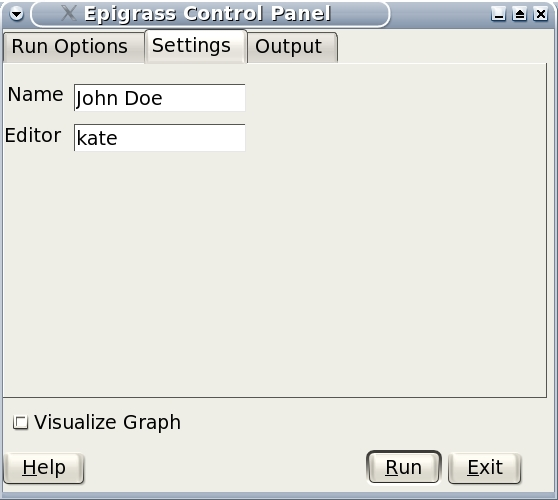
\includegraphics[scale=0.7]{guiset.jpg}
% guiset.jpg: 72dpi, width=19.68cm, height=17.64cm, bb=0 0 558 500
	\caption{Second tab of the GUI.}
	\label{fig:guiset}
\end{figure}

\subsection{Utilities}
In the Utilities tab, you can get feed back from the simulator. Especially during long simulation runs, it is good to know how it is progressing. During the simulation, text messages regarding the status of the simulation are written to the text box on the left. 
\begin{figure}
	\centering
%	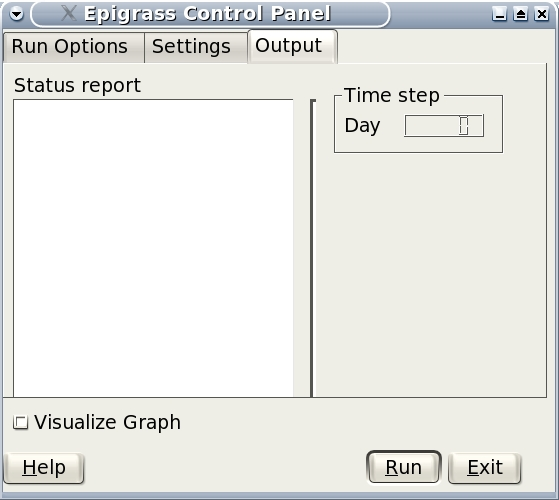
\includegraphics[scale=0.7]{guiout.jpg}
% guiout.jpg: 72dpi, width=19.72cm, height=17.64cm, bb=0 0 559 500
	\caption{Third tab of the GUI}
	\label{fig:guiout}
\end{figure}

On the right, there is a button for backing up the data base and another for opening the report generated by the last simulation. Since report PDFs ar stored in folder directly below the ones on which the simulation is started, older reports should still be accessible and can be opened directly by selecting the desired report using the operating system's file manager.

\subsection{Visualization}
The fourth tab of the GUI is the visualization Tab. This tab was designed for playing animations of any simulation data that is stored in the database. Pressin the \texttt{Scan DB} button, causes the available tables in the  epigrass database to be listed in the \texttt{Simulations stored} combo box. The user can then select one of these simulations to visualize.

Once the \texttt{Start animation} button is pressed, a graphical display window pops up, and the simulation is replayed at a speed given by the frame rate set by the user  or the maximum speed of the computer (whichever is smaller). In the animation, the nodes of the network are represented by boxes whose volume is given by the number of infected at each node. The node colors are as following: Green for uninfected nodes, and red to blue for infected nodes. bright red for for first infected node with the nodes becoming infected later assuming a color with progressively more blue.


Maps can also be selected from the \texttt{Maps availabled combo box} to be used as background for the network display. The maps must be in the GRASS ascii vectorial format and have coordinates compatible with those given to the nodes of the simulation.

\subsection{Operation}
After all the information has been entered and checked on the GUI, you can press the \texttt{Run} button to start the simulation or the \texttt{Exit} button. When the \texttt{Run} button is pressed, the \texttt{.epigrassrc} file is updated with all the information entered in the gui. If the \texttt{Exit} button is pressed, all information entered since the last time the \texttt{Run} button was pressed is lost.



\chapter{Interpreting the output}   \label{cap:analysis}
\lettrine{T}he outputs of EpiGrass simulations were designed to be as flexible as possible. Beside the automated report generation which serves as an overview of the model and its results, raw data is also made available for ready utilization from other softwares such as R and Grass.

\section{Visualization}

On the graphical user interface, if you check the box \texttt{Visualize Graph}, a 3D display opens up when the simulation is started. This display will plot the network on the map (if a map is available). As the simulation progresses, the nodes  change color from green to red as the localities become infected. Localities that get infected later are assigned a different shades of red which will tend to become blue as the time progresses. This way the sequence of infection remains visible throughout the simulation by means of this color scale.

The visualization module can also be invoked independently of the simulation to review the dynamics of simulation data stored on the database. This way, any previous simulation can be reviewed at any time. It is also recommended that simulataneous visualization be turned off to speed up calculations.  

Currently, the visualization module displays only the temporal dynamics of infection with the number of infected individuals in each infected locality is represented by the size of the node object in the network plot. 

\section{Database}
The simulated time series are stored in a MySQL table in the database epigrass: E, I, S, incidence (L), together with time, geocode and coordinates. The table is named after the filename of the script and date and time of the simulation.

Epigrass provides an R script for importing the data into R for further analysis and display \footnote{see appendix \ref{cap:introR}}.     

\section{Epidemiological descriptors}
At the end of the simulation, Epigrass calculates a set of epidemiological stats. These stats are presented to the user in two ways: as a .csv table that can be imported by R or any other statistical package; and as a written (PDF format) report.  Stats include descriptors of the epidemic dynamics at the whole graph level and also node-specific stats:
\paragraph*{Graph-level stats:}
\begin{description}
\item[Epidemic pop size] Total number of cases in the whole graph during the simulation. 
\item[Epidemic size] Total number of cities that had authoctonous transmission during the simulation. 
\item[Mean epidemic speed] Average number of new localities infected per time step.
\item[Epidemic Duration] Time between the first and last case.
\item[Median survival] Time to reach 50\% of the cities.
\item[Vaccinated] Total number of vaccinated individuals.
\item[Quarantined] Total number of quarantined individuals.
\item[Pass] Total number of infected individuals travelling through the network.
\item[Top ten nodes] Main cities in terms of number of infected.
\item[First ten nodes] First ten infected cities.
\end{description}

At the site scale, the report returns for each site $i$:
\begin{description}
\item[Incidence] Accumulated number of new cases per time step
\item[Local epidemic size] Total number of cases that occurred in the site during the simulation.
\item[Infectious arriving] Number of infected individuals arriving per time step


%\item[Local outbreak start point($t_i$)] Time step of first authoctonously transmitted infection in $i$.
%\item[Local arrival ($y_i$)] Total number of infected individuals that visited $i$ during the simulation.
%\item[Speed of spread($\sigma_1$)] Number (or proportion) of new localities infected per time step
%\item[Speed of spread($\sigma_2$)] Number (or proportion) of new localities infected per time step, weighed by population size of these localities (?).
%\item[Speed of propagation($\sigma_3$)] Velocitity of propagation in $km^2/day$, where velocity of propagation is defined as a velocity $c$ so that, if you run faster than $c$, you leave the epidemi behind and, if you run slower than $c$, the epidemic will eventually surrounds you (Rass and Radcliff. Spatial Deterministic epidemics, livro).
%\item[Speed of propagation($\sigma_4$)] Velocity of movement of the centroid of the epidemic region.
%\item{Mean direction of spread}
%\item{}   
\end{description}

\section{Network Descriptive Statistics}
EpiGrass automatically calculates and displays descriptive statistics about the network structure in Reports 1 and 3.
\subsection{Basic Numbers}
       \begin{description}
        \item[Order (Number of Nodes):] The Number of localities the network is composed of.
        \item[Size (Number of Edges):] The number of transportation routes connecting any pair of nodes. 
	\item [Eulerian:] Can be yes or No depending on if the networkgrap is eulerian o not. A Eulerian graph contains a circuit (Eulerian circuit) which includes all nodes an edges of the graph.
	\item [Traversable:]Can be Yes or No depending on if the network graph contains an Eulerian trail, i.e. a trail tht includes all the nodes an edges of the graph.   
        \end{description}
        
	\subsection{Shortest-path Distribution}
	In a network there are frequently more than one path from locality A to locality B. Of these possible  routes, the shortest path is the most important when dealing with epidemic processes over networks.
	
        A network distance Matrix can be calculated whose elements represent the number of edges separating any pair of nodes via the shortest path between them. From this matrix a histogram of the Shortest-paths lengths can be generated which gives us an idea of give us an idea of how fast an epidemic would spread in our network, if distance was the only factor.
        
        
        \subsection{Conectivity Matrix}
        The most basic measure of accessibility involves network connectivity
        where a network is represented as a connectivity matrix(figure \ref{fig:cm}), which 
        expresses the connectivity of each node with its adjacent nodes. 
        
        The number of columns and rows in this matrix is equal to the number 
        of nodes in the network and a value of 1 is given to each cell representing a directly connected pair and a value of 0 to each cell representing an unconnected pair. The summation of this matrix, along its rows or collumns, provides a very 
        basic measure of node accessibility, also known as the degree of a node.
        \begin{figure}[h]
        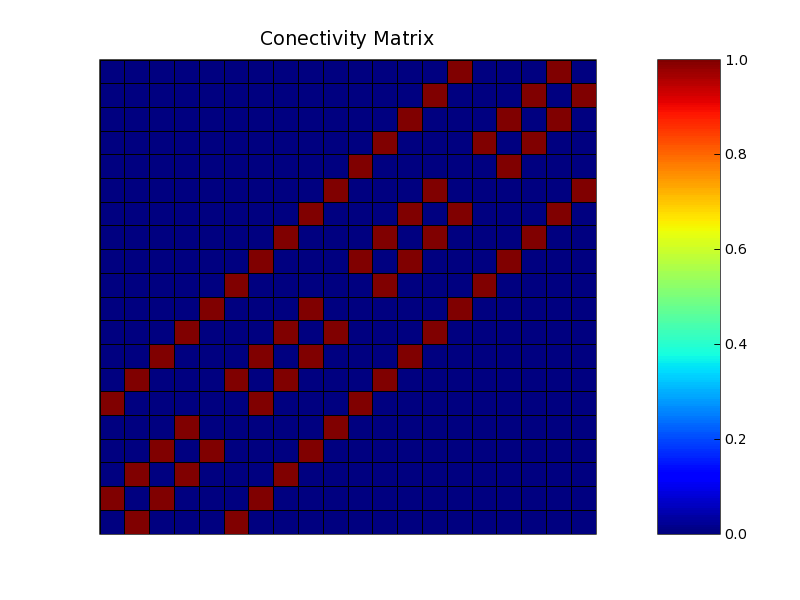
\includegraphics[scale=0.6]{cm.png}
        \centering
        \caption{Connectivity matrix of a simple grid network}
        \label{fig:cm}
        \end{figure}
        
        indices = r"""
        \subsection{Number of Cycles}
	A cycle is a circular path, meaning that in ends wher it started, that does not repeat an edge. The index presented here is the maximum number of independent cycles in a network.
	
        This number ($u$) is estimated by knowing the number of nodes ($v$), 
        links ($e$) and of sub-graphs ($p$);
        
        Trees and simple networks will have a value of 0 since they have 
        no cycles. 
        The more complex a network is, the higher the value of u, 
        so it can be used as an indicator of the level of development 
        of a transport system.
        
        $$ u=e-v+p$$
        
        \subsection{Wiener Distance}
        The Wiener distance is the sum of all the shortest distances in the network.
        
        $$D_W =\sum_{i=1}^v\sum_{j=1}^i\;D_{ij}$$
	
	where $D$ is the Shortest distance matrix.
        
        \subsection{Mean Distance}
        The mean distance of a network is the mean of of the set of shortest paths, 
        excluding the 0-length paths.
        
        $$\bar{D}=\frac{1}{v}\sum_{i=1}^v\sum_{j=1}^i\;D_{ij}\;\;\; \forall\; D_{ij}\neq0$$ 
        \subsection{Network Diameter}
        The diameter of a network is the longest element of the shortest paths set.
        
        \subsection{Length of the Network}
        The length of a network is the sum in metric units (e.g., km) of all the edges in the network.

        \subsection{Weight of the Network}
        The weight of a network is the weight of all nodes in the graph ($W(N)$), which is the summation 
        of each node's order ($o$) multiplied by 2 for all orders above 1.
        
        $W(N)=$
        \subsection{Iota ($\iota$) Index}
        The Iota index measures the ratio between the network and its weighed vertices. 
        It considers the structure, the length and the function 
        of a network and it is mainly used when data about traffic 
        is not available. 
        
        It divides the length of a network (L(N)) by its weight (W(N)). 
        The lower its value, the more efficient the network is. 
        This measure is based on the fact that an intersection 
        (represented as a node) of a high order is able to handle 
        large amounts of traffic. 
        
        The weight of all nodes in the network (W(N)) is the summation 
        of each node's order (o) multiplied by 2 for all orders above 1.
        
        $\iota=\dfrac{L(N)}{W(N)}=$
        \subsection{Pi ($\Pi$) Index}
        The Pi index represents the relationship between the 
        total length of the network L(N)
        and the distance along the diameter D(d). 
        
        It is labeled as Pi because of its similarity with the 
        trigonometric $\Pi$ (3.14), which is expressing the ratio between 
        the circumference and the diameter of a circle. 
        
        A high index shows a developed network. It is a measure 
        of distance per units of diameter and an indicator of 
        the  shape of a network.
        
        $\Pi=L(N)/D(d)=$
        \subsection{Beta ($\beta$) Index}
        The Beta index
        measures the level of connectivity in a network and is 
        expressed by the relationship between the number of 
        edges (e) over the number of nodes (v). 
        
        Trees and simple networks have Beta value of less than one. 
        A connected network with one cycle has a value of 1. 
        More complex networks have a value greater than 1. 
        In a network with a fixed number of nodes, the higher the 
        number of links, the higher the number of paths possible in 
        the network. Complex networks have a high value of Beta.
        
        $\beta = $
        \subsection{Alpha ($\alpha$) Index}
        The Alpha index is a measure of connectivity which evaluates
        the number of cycles in a network in comparison with the maximum 
        number of cycles. The higher the alpha index, the more a network 
        is connected. Trees and simple networks will have a value of 0. 
        A value of 1 indicates a completely connected network. 
        
        Measures the level of connectivity independently of the number of
        nodes. It is very rare that a network will have an alpha value of 1, 
        because this would imply very serious redundancies.
        
        $\alpha=$
        \subsection{Gamma ($\Gamma$) Index}
        The Gamma index is a A measure of connectivity that considers
        the relationship between the number of observed edges and the
        number of possible edges. 
        
        The value of gamma is between 0 and 1 where a value of 1 
        indicates a completely connected network and would be extremely 
        unlikely in reality. Gamma is an efficient value to measure 
        the progression of a network in time.
        
        $\Gamma=$
        \subsection{Site Oriented Statistics}
        \begin{description}
                \item[Centrality:]Also known as closeness. A measure of global centrality, is the 
                inverse of the sum of the shortest paths to all other nodes
                in the graph.
                \item[Degree:]The order (degree) of a node is the number of its attached links 
                and is a simple, but effective measure of nodal importance. 
                
                The higher its value, the more a node is important in a graph 
                as many links converge to it. Hub nodes have a high order, 
                while terminal points have an order that can be as low as 1. 
                
                A perfect hub would have its order equal to the summation of 
                all the orders of the other nodes in the graph and a perfect 
                spoke would have an order of 1.
                \item[Theta Index:]Measures the function of a node, that is the average
                amount of traffic per intersection. The higher theta is,
                the greater the load of the network.
                \item[Betweeness:]Is the number of times any node figures in the the shortest path
                between any other pair of nodes.
        \end{description}
       

\section{Example}




\appendix
\chapter{Example of Model Definition Script} 
\label{script}

\begin{lstlisting}[basicstyle=\footnotesize,language=Python, frame=trBL, caption= ,label=]

################################################################
#
#  EPIGRASS -Model Definition
#  This script describes model and parameters specified
#  by the user.
#  It can be edited by the user directly, by means of a text editor.
#  WARNING: No variables may be removed, even if not used by the chosen model . 
#  Any comments added by the user must be preceeded  by the symbol #
#
################################################################
################################################################

#==============================================================#
[THE WORLD]
#==============================================================#
# Here you add iformation about the files that described the world the model is enclosed
# "Location" is the GRASS location with the maps describing the area.
# "vector layer" is the map layer that will be used as a background for the network display
# "sites" and "edges" are the files that describe the topology of the network (see Documtntation)

location = BRASIL
vector layer = Limite_politico_administrativo
sites = sitios2.csv
edges = edgesout.csv

#==============================================================#
[EPIDEMIOLOGICAL MODEL]
#==============================================================#
#model types available: SIS, SIS_s ,SIR, SIR_s, SEIS, SEIS_s, SEIR, SEIR_s, 
# SIpRpS, SIpRpS_s,SIpR,SIpR_s(see documentation for description)
modtype = SIR

#==============================================================#
[MODEL PARAMETERS]
#==============================================================#

#  They can be specified as constants or as functions of global or 
#  site-specific variables. these site-specific variables, are provided
#  in the sites file. All the numbers given after the geocode (4th column)
#  are collected into the values tuple.
# Examples:
# beta = 0.001
# beta=values[0] #assigns the first element of values to beta 
# beta=0.001*values[1]

beta = 0.4   #transmission coefficient (contact rate * transmissibility)
alpha = 1  # clumping parameter
e = 1   # inverse of incubation period
r = 0.1   # inverse of infectious period
delta = 1  # probability of acquiring full immunity [0,1]
B = 0           # Birth rate
w = 0           # probability of immunity waning [0,1]
p = 0           # Probability of a recovered become infected per time step [0,1]


#==============================================================#
[INITIAL CONDITIONS]
#==============================================================#
# Here, the number of individuals in each epidemiological
# state (SEI) is specified. They can be specified in absolute
# or relative numbers.
# N is the population size of each site.
# The rule defined here will be applied equally to all sites.
# For site-specific definitions, use EVENTS (below)
# Examples:
# S,E,I = 0.8*N, 10, 0.5*E
# S,E,I = 0.5*N, 0.01*N, 0.05*N
# S,E,I = N-1, 1, 0
S = N
E = 0
I = 0

#=============================================================#
[EPIDEMIC EVENTS]
#=============================================================#
# Specify isolated events.
#  Localities where the events are to take place should be Identified by the geocode, which 
#  comes after population size on the sites data file.
#  All coverages must be a number between 0 and 1.
#  Seed : [('locality1's geocode', n),('locality2's geocode', n)]. 
#  N infected cases will be added to locality at time 0.
#  Vaccinate: [('locality1's geocode', time, coverage),('locality2's geocode', time, coverage)] 
#  Quarantine: [(locality1's geocode,time,coverage), (locality2's geocode,time,coverage)]
seed = [(230440005,1)] #Fortaleza
Vaccinate = [(355030800, 31, 0)] #Sao Paulo
Quarantine = [(355030800,20,0)]
#Screening = (locality, time, coverage)#screening for sick people on aiports bus stations
#Vector_control = (locality, time, coverage)
#Treatment = (locality, time, coverage)
#Prophylaxis = (locality, time, coverage)

#==============================================================#
[TRANSPORTATION MODEL]
#==============================================================#
# If doTransp = 1 the transportation dinamics will be included. Use 0 here only for debugging purposes.
doTransp = 1

# NEIGHBORHOOD DEFINITION


# SPATIAL COUPLING


#==============================================================#
[SIMULATION AND OUTPUT]
#==============================================================#

# Number of steps
steps = 200

# Output dir
outdir = ~/data

# Output file
outfile = simul.dat

# Database Output
# MySQLout can be 0 (no database output) or 1
MySQLout = 1 

# Graphical outputs
draw map = 1

# Report Generation
# The variable report can take the following values:
# 0 - No report is generated.
# 1 - A network analysis report is generated in PDF Format.
# 2 - An epidemiological report is generated in PDF Format.
# 3 - A full report is generated in PDF Format.
# siteRep is a list with site geocodes. For each site in this list, a detailed report is apended to the main report.
report = 0
siteRep = [230440005,355030800]

#Batch Run
#  list other scripts to be run in after this one. don't forget the extension .epg
#  model scripts must be in the same directory as this file or provide full path.
#  Example: Batch = ['model2.epg','model3.epg','/home/jose/model4.epg']
Batch = []

################################################################
################################################################



\end{lstlisting}
%\include{shortintroGRASS}
%\include{shortintroSQL}
\chapter{Using R to Analyze EpiGrass' Data}\label{cap:introR} 
Depending on the size of your network or the number of scenarions being simulated on a given network within EpiGrass, A large ammount of data is generated as output. This data is stored, by default on a MySQL database named epigrass.

On this appendix, we illustrate how to access this data on the MySQL server an do sme simple analysis using the statistical package R. The R statistical package (\url{http://www.r-project.org}) is an incredibly resourceful environment for data management and analysis. 

\section{Accessing The MySQL server}
Before we can access the database and retrieve our data there are some preliminary steps that must be performed. First and foremost, we need to learn how to start the R system. Just open a console window and type \texttt{R} as shown on listing \ref{lst:startR}.
\begin{lstlisting}[language=Ksh,basicstyle=\footnotesize,frame=trBL, caption=Starting R ,label=lst:startR]
$ R
R : Copyright 2004, The R Foundation for Statistical Computing
Version 2.0.1  (2004-11-15), ISBN 3-900051-07-0

R is free software and comes with ABSOLUTELY NO WARRANTY.
You are welcome to redistribute it under certain conditions.
Type 'license()' or 'licence()' for distribution details.

R is a collaborative project with many contributors.
Type 'contributors()' for more information and
'citation()' on how to cite R or R packages in publications.

Type 'demo()' for some demos, 'help()' for on-line help, or
'help.start()' for a HTML browser interface to help.
Type 'q()' to quit R.

>                       
\end{lstlisting}

Very well, Now you are running R. R has a modular architecture that allows the user to specify the tools he/she desires to use on a given session. In order to access the MySQL database server and retrieve our data, we will need some special tools from R's vast colection of modules (also called packages). Listing \ref{lst:Rlib}, shows how to load the packages needed.
\begin{lstlisting}[language=R,basicstyle=\footnotesize,frame=trBL, caption=Loading required packages.,label=lst:Rlib]
> library(DBI)
> library(RMySQL)
\end{lstlisting}

To connect to a database server we need to tell R the type of server we will be connecting to, and open a connection to it (listing \ref{lst:Rsql}). 
\begin{lstlisting}[language=R,basicstyle=\footnotesize,frame=trBL, caption=Specifying the type of server and opening a connection.,label=lst:Rsql]
> drv <- dbDriver("MySQL")
> con <- dbConnect(drv, username='epigrass',password='epigrass', host='localhost',dbname='epigrass')
\end{lstlisting}

Once we have a connection to the database it works as a two-way communications pipeline between R and the MySQL server. Through this connection we can send SQL commands to the Server and retrieve the results of these commands. 

Fortunately, the RMySQL package has many common SQL statements packed into easy to remember commands. Listing \ref{lst:Rlisttbl} shows us how to find out the tables available at the epigrass database. This is a very useful command for us because the results of each simulation completed in EpiGrass is stored in a separate table whose title is contains a reference to when it was ran. So, after running a few simulations with the demo model mesh, we will end up with a list of tables similar to the one shown on listing  \ref{lst:Rlisttbl}.
\begin{lstlisting}[language=R,basicstyle=\footnotesize,frame=trBL, caption=Listing existing tables. ,label=lst:Rlisttbl]
> tables<-dbListTables(con)
> tables
[1] "localidades"                   "mesh_Mon_Feb_14_111026_2005"
[3] "mesh_Tue_Feb_15_144139_2005"   "mesh_Tue_Feb_15_171743_2005"
[5] "mesh_Tue_Feb_15_172037_2005"   "mesh_Tue_Feb_15_172134_2005"
\end{lstlisting}

After we identify which set of data(table) we want to work with, we can read the into a data frame, a very versatile data structure of R.

\begin{lstlisting}[language=R,basicstyle=\footnotesize,frame=trBL, caption= ,label=lst:Rrdtbl]
> results<- dbReadTable(con,tables[2])
> names (results)
[1] "geocode" "time"    "E"       "I"       "S"
\end{lstlisting}

On line 1 of listing \ref{lst:Rrdtbl}, we read the second table of our database into a data frame object called \texttt{results}. The \texttt{names} command, lists the names of the variables contained in that data frame.

\section{Visualizing the Data}
Once we have have the data inside R there countless ways in which we can manipulate and visualize it. For the first plot we will need to load another package called \texttt{lattice}. 
\begin{lstlisting}[language=R,basicstyle=\footnotesize,frame=trBL, caption= ,label=]
> library(lattice)
> xyplot(I+E+S~time|geocode,type="l",data=results)
\end{lstlisting}

\bibliographystyle{amsalpha}
\bibliography{userguide}

\backmatter
\printindex

\end{document}
